\documentclass[12pt,a4paper]{report}
\usepackage[utf8]{inputenc}
\usepackage{parskip}
\usepackage{pdfpages}
\usepackage{amsmath}
\usepackage{url}
\usepackage{caption}
\usepackage{subcaption}
\usepackage[inkscapeformat=png]{svg}
\usepackage{adjustbox}
\usepackage{algorithm}  % algorithm
\usepackage{algpseudocode}  % algorithm
\renewcommand{\algorithmicrequire}{\textbf{Input:}}
\renewcommand{\algorithmicensure}{\textbf{Output:}}

\def\UrlBreaks{\do\/\do-}

\usepackage{listings}
\lstset{
basicstyle=\small\ttfamily,
columns=flexible,
breaklines=true
}

\usepackage{graphicx}
\graphicspath{ {./diss_images/} }

\begin{document}

%%%%%%%%%%%%%%%%%%%%%%%%%%%%%%%%%%%%%%%%%%%%%%%%%%%%%%%%%%%%%%%%%%%%%%%
% Title
%TC:ignore
\pagestyle{empty}
\pagenumbering{gobble}

\vspace*{60mm}
\begin{center}
\Huge
\textbf{Cycle routes: connecting the network}

\vfill
\large
Jiaxin Wang \\[3mm]
Supervisor: Dr Michael Young \\[3mm]
University of St Andrews \\[3mm]
\today  % today's date
\end{center}
\thispagestyle{empty}

\pagestyle{plain}
\chapter*{Abstract}
This project aims to build an automated process to analyse the cycling infrastructure of an area and produce recommendations for additional cycle-friendly paths. We have built a three-layer system to fetch data from OpenStreetMap, analyse the data and produce a graph annotated with data relevant to cycling. From the graph, we have implemented various strategies to suggest where improving the cycling infrastructure would have the greatest impact. The process was applied to three areas: St Andrews and Dundee in Scotland, as well as Houten in the Netherlands. The effectiveness of the suggested paths were evaluated using metrics relevant to connectivity.

\chapter*{Declaration}
I declare that the material submitted for assessment is my own work except where credit is explicitly given to others by citation or acknowledgement. This work was performed during the current academic year except where otherwise stated.

The main text of this project report is 10,584 words long, including project specification and plan.

In submitting this project report to the University of St Andrews, I give permission for it to be made available for use in accordance with the regulations of the University Library. I also give permission for the title and abstract to be published and for copies of the report to be made and supplied at cost to any bona fide library or research worker, and to be made available on the World Wide Web. I retain the copyright in this work.

\clearpage
\setcounter{page}{1}
\pagenumbering{roman}

\tableofcontents

\listoffigures

\newpage
\pagenumbering{arabic}
%TC:endignore

\chapter{Introduction}
In this chapter, we will discuss the motivation behind this project. We will present a list of aims and objectives, and give a brief overview of the structure of this report.

\section{Motivation}
With the climate crisis, there has been a big push from many facets of society to reduce car usage~\cite{CHAPMAN2007354}. Encouraging more people to cycle over short distances instead of driving would be a big step towards reaching that goal. A study by Sloman et al. suggests that investment in cycling leads to increased cycle levels~\cite{Sloman2009}. Many cities and towns have invested money into creating new cycling infrastructure, such as cycle paths alongside roads or standalone cycleways. Public budgets are always squeezed, so it is important to prioritize infrastructure improvements in the places where they would have the most impact. 

Given the street map data of an area, it is possible to analyse the existing cycle infrastructure and identify the places where improvement is most needed. For each path in the street map, we can evaluate its suitability for safe cycling using data such as speed limits and cycle lanes. For example, a designated cycle lane is considered to be more cycle-friendly than a busy main road. If we consider the subgraph which consists of cycle-friendly paths only, we could potentially identify isolated areas that are disconnected from the rest of the graph. It might be safe to cycle within each area, but it could be difficult for cyclists to commute from one area to another. An improvement to the cycle network would be to add cycle-friendly paths to connect such areas.

There are many network analysis tools implemented in various programming languages, but users without any technical expertise could struggle to apply such tools to the map data. There is a need for a system which allows less technical users to analyse street maps with respect to cycling infrastructure.

\section{Aims and Objectives} \label{sec:aims}
The aim of this project is to implement an automated system which provides recommendations for additional cycle paths by analysing the map of St Andrews. The system should be extensible to other areas without any manual data processing.

The primary objectives are listed below:
\begin{enumerate}
    \item Develop an automated process that turns the OpenStreetMap data for an area into a graph annotated with data relevant to cycle accessibility and apply this to St Andrews
    \item Develop a set of configurable heuristics to determine whether a route is cycle friendly
    \item Apply the heuristics to highlight disconnected components in the cycle-friendly subgraph
    \item Consider other properties of the graph, such as k-connectivity and induced subgraphs, to produce other findings relevant to cycling
    \item Suggest the most efficient paths to add to increase the connectedness of the subgraph
\end{enumerate}

A list of secondary objectives are considered, with lower priority than the primary objectives:
\begin{enumerate}
    \item Apply this analysis process to another similar area and assess how well the automated process works for areas it was not designed for
    \item Apply the analysis process to a larger area to evaluate the scalability of the technique
    \item Consider the cost of adding new paths when making suggestions
\end{enumerate}

\section{Report Structure}
Chapter \ref{chapter:context} gives an overview of graph theory which is relevant to this project and related work in this area. Chapter \ref{chapter:design} concerns the structure of the system. The implementation of the system is discussed in Chapter \ref{chapter:impl}, with focus on high-level algorithms. In Chapter \ref{chapter:eval}, we evaluate the success and limitations of the system and compare it against existing approaches. Chapter \ref{chapter:concl} summarizes the project and discusses potential future work.

\chapter{Context Survey}\label{chapter:context}
This project is closely related to graph theory, and research has been done in this field. In Section \ref{sec:graph_theory}, we will look into some important concepts in graph theory. Section \ref{sec:related_work} gives an overview of related work in this area. Tools and libraries that may be relevant to this project are discussed.

\section{Graph Theory} \label{sec:graph_theory}
A \textit{graph} $G=(V,E)$ is a mathematical structure which consists of a set of vertices $V$ and a set of edges $E$, where each edge is a pair of vertices in $V$~\cite{chartrand}. A graph $H$ is called a \textit{subgraph} of $G$ if $V(H) \subseteq V(G)$ and $V(H) \subseteq V(G)$. A \textit{weighted} graph $G=(V,E,W)$ is a graph where each edge is assigned a weight value, and the weight mapping is stored in $W$. A \textit{directed} graph is a graph where each edge is directed, whereas an \textit{undirected} graph is a graph where edges have no direction. A \textit{hypergraph} is denoted by $H=(V;\mathcal{E})$, where $V$ is a set of vertices and $\mathcal{E}$ is a set of hyperedges. Each hyperedge joins any number of vertices.

\begin{figure}[ht]
    \centering
    \begin{subfigure}[ht]{0.33\textwidth}
        \centering
        \includegraphics[width=\textwidth]{diss_images/context/weighted.png}
        \caption{A weighted graph}
        \label{fig:weighted}
    \end{subfigure}
    \hfill
    \begin{subfigure}[ht]{0.32\textwidth}
        \centering
        \includegraphics[width=\textwidth]{diss_images/context/directed.png}
        \caption{A directed graph}
        \label{fig:directed}
    \end{subfigure}
    \hfill
    \begin{subfigure}[ht]{0.32\textwidth}
        \centering
        \includegraphics[width=\textwidth]{diss_images/context/undirected.png}
        \caption{An undirected graph}
        \label{fig:undirected}
    \end{subfigure}
       \caption{Three simple graphs}
       \label{fig:three graphs}
\end{figure}

Three simple graphs are demonstrated in Figure~\ref{fig:three graphs}. Figure~\ref{fig:weighted} shows a weighted graph with $V = \{A, B, C, D\}$ and $E = \{AC, BC, CD\}$, where the weight of each edge is labelled next to the edge. An example of a directed graph and an undirected graph are shown in Figure~\ref{fig:directed} and \ref{fig:undirected} respectively. Figure~\ref{fig:fanoplane} shows the Fano plane, which is an example of a hypergraph. It contains seven vertices as labelled on the diagram, and it has seven hyperedges: $\mathcal{E} = \{123, 145, 167, 246, 257, 347, 365\}$.

\begin{figure}[ht]
    \centering
    \includegraphics[width=0.3\textwidth]{diss_images/context/fanoplane.png}
    \caption{The Fano plane from Wikipedia~\cite{WikipediaEN:fanoplane}}
    \label{fig:fanoplane}
\end{figure}

Street maps can be considered as a type of hypergraph, where locations on the map are the vertices and streets joining various locations are the hyperedges. However, most implementations of graph algorithms are designed for graphs instead of hypergraphs. A hypergraph can be converted into a graph when we know the order of the nodes on each hyperedge. We make each hyperedge into a set of edges, where each node along the hyperedge is part of at most two edges: one with its predecessor if it exists, and one with its successor if it exists. This process will create many edges, and to reduce the computational space it may be sensible to disregard the nodes that only appear in one hyperedge, since these nodes are irrelevant for connectivity.

In a street map we do know the order of the nodes along the hyperedges, since each way consists of an ordered list of nodes. Therefore, we can create a graph from the street map hypergraph, and analyse the subgraph which only consists of cycle-friendly routes. We can then identify isolated areas in this subgraph, where there are no connecting edges between the isolated area and other parts of the graph. In the following sections, we present some graph algorithms which can be useful in our task.

\subsection{Connectivity}
The \textit{vertex-connectivity} of a graph is defined as the minimum number of vertices that need to be removed to result in a disconnected graph, and the \textit{edge-connectivity} of a graph is the minimum number of edges that need to be removed to result in a disconnected graph~\cite{buckley1990distance}. A graph is \textit{k-vertex-connected} if it has vertex-connectivity $k$.

\begin{figure}[ht]
    \centering
    \includegraphics[width=0.25\textwidth]{diss_images/context/connectivity.png}
    \caption{A 4-connected graph from Wikipedia~\cite{WikipediaEN:Connectivity}}
    \label{fig:connectivity4}
\end{figure}

Figure~\ref{fig:connectivity4} shows a 4-vertex-connected graph. To separate the graph into two isolated subgraphs, the minimum number of vertices that need to be removed is four. For example, after removing the two left-most vertices and the two right-most vertices, we obtain two disconnected subgraphs, each of which consists of one vertex and no edges. 

The more connected the cycle-friendly subgraph is, the easier it is to get around the area with bicycles. An intuition to improve the cycle infrastructure would be to add paths that would increase the connectivity of the graph.

\subsection{Graph traversal}
If a graph $S$ is a maximally connected subgraph of graph $G$, then $S$ is a $component$ of $G$~\cite{citeulike:395714}. We can analyse the connected components in the cycle-friendly graph and add edges between them to connect smaller cycle-friendly regions into a large cycle-friendly component. The set of components in an undirected graph can be found by traversing the graph. Running a search from a node $n$ will give us all the reachable nodes from $n$, which form a component containing $n$. Therefore, running search algorithms from each unvisited node will yield the set of connected components in a graph.

There are two common examples of search algorithms, namely \textit{breadth-first search} (BFS) and \textit{depth-first search} (DFS). The BFS algorithm works by visiting each node in turn, starting with the closest nodes to origin and keeping the unvisited neighbours in a queue. The DFS algorithm runs in the same way, except it uses a stack to explore each branch in full before backtracking.

\subsection{Shortest path}
In order to measure the cost of cycling, we can look at the cost of the shortest paths. There are many algorithms for finding the shortest paths between nodes in a graph, perhaps the most famous of which is Dijkstra's shortest path algorithm~\cite{dijkstra1959note}. It takes a starting point and works out the shortest path to all other reachable nodes. The algorithm is outlined in Algorithm~\ref{alg:dijkstra}~\cite{WikipediaEN:dijkstra}.

\begin{algorithm}
\caption{Dijkstra's Algorithm}\label{alg:dijkstra}
\begin{algorithmic}
\Function{Dijkstra}{$Graph$, $source$}
    \State let $Graph = (V, E, W)$
    \For{$v$ in $V$}
        \State $dist[v]\gets \infty$
        \State $prev[v]\gets undefined$
        \State add $v$ to $Q$
    \EndFor
    \State $dist[source]\gets 0$
    \While{$Q$ is not empty}
        \State $u\gets$ vertex in $Q$ with min $dist[u]$
        \State remove $u$ from $Q$
        \For{neighbour $v$ of $u$ still in $Q$}
            \State $alt \gets dist[u] + E(u, v)$
            \If{$alt < dist[v]$}
                \State $dist[v]\gets alt$
                \State $prev[v]\gets u$
            \EndIf
        \EndFor
    \EndWhile
    \State \Return $dist, prev$
\EndFunction
\end{algorithmic}
\end{algorithm}

Consider the graph in Figure~\ref{fig:dijkstra_example}~\cite{abba2022}, we can use Dijkstra's algorithm to find the shortest distance from node A to every other node. During the process, we would keep a priority queue, which stores the shortest distance so far to a node from node A, with the smallest distance being at the front of the queue. After visiting the node A, the priority queue would look like this:
\[C=2, B=4, D=\infty, E=\infty\]

\begin{figure}[ht]
\centering
\includegraphics[width=0.5\textwidth]{diss_images/context/dijkstra.png}
\caption{An undirected graph taken from freeCodeCamp~\cite{abba2022}}
\label{fig:dijkstra_example}
\end{figure}

This is because the shortest distance from A to B is 4, from A to C is 2. Then we choose a new unvisited node from the front of the priority queue, in this case, C. After visiting the node C, we can update the priority queue:
\[B=3, D=\infty, E=\infty\]

C is now visited, so it is removed from the priority queue. Since $2+1 \leq 4$, the shortest distance between AB is updated to be 3. The next node to be visited is B, which is at the front of the priority queue. After visiting B, we have:
\[E=5, D=6\]

And after visiting E, we have:
\[D=6\]

Finally, D is visited and there are no unvisited nodes left. We have computed that the shortest distance from A to every other node:
\[B=3, C=2, D=6, E=5\]

Another famous graph algorithm is Prim's algorithm, which finds the minimum spanning tree for a weighted undirected graph. The minimum spanning tree of a graph is defined to be the tree with the minimum total edge weights which connects all vertices~\cite{Pettie2008}. An example of a minimum spanning tree is shown in Figure~\ref{fig:mst_example}. In our task of improving the cycling infrastructure, we can use it to identify the paths that connect all areas with the lowest total distance and improve the graph based on this metric.

\begin{figure}[ht]
\centering
\includegraphics[width=0.5\textwidth]{diss_images/context/MST.png}
\caption{A minimum spanning tree example from Wikipedia~\cite{WikipediaEN:MST}}
\label{fig:mst_example}
\end{figure}

\section{Related Work} \label{sec:related_work}
\subsection{OpenStreetMap}
OpenStreetMap~\cite{OpenStreetMap} is an open, user-generated map database. It is licensed under the Open Data Commons Open Database Licence~\cite{odbl}. There are four types of data in OSM~\cite{9119753}:
\begin{itemize}
    \item A node, which is a location on the Earth's surface with longitude and latitude
    \item A way, which is an ordered list of nodes representing roads and objects along the road
    \item A relation, which specifies the association among objects
    \item A tag, which is a key-value pair regarding information about an object
\end{itemize}

\begin{figure}[ht!]
\centering
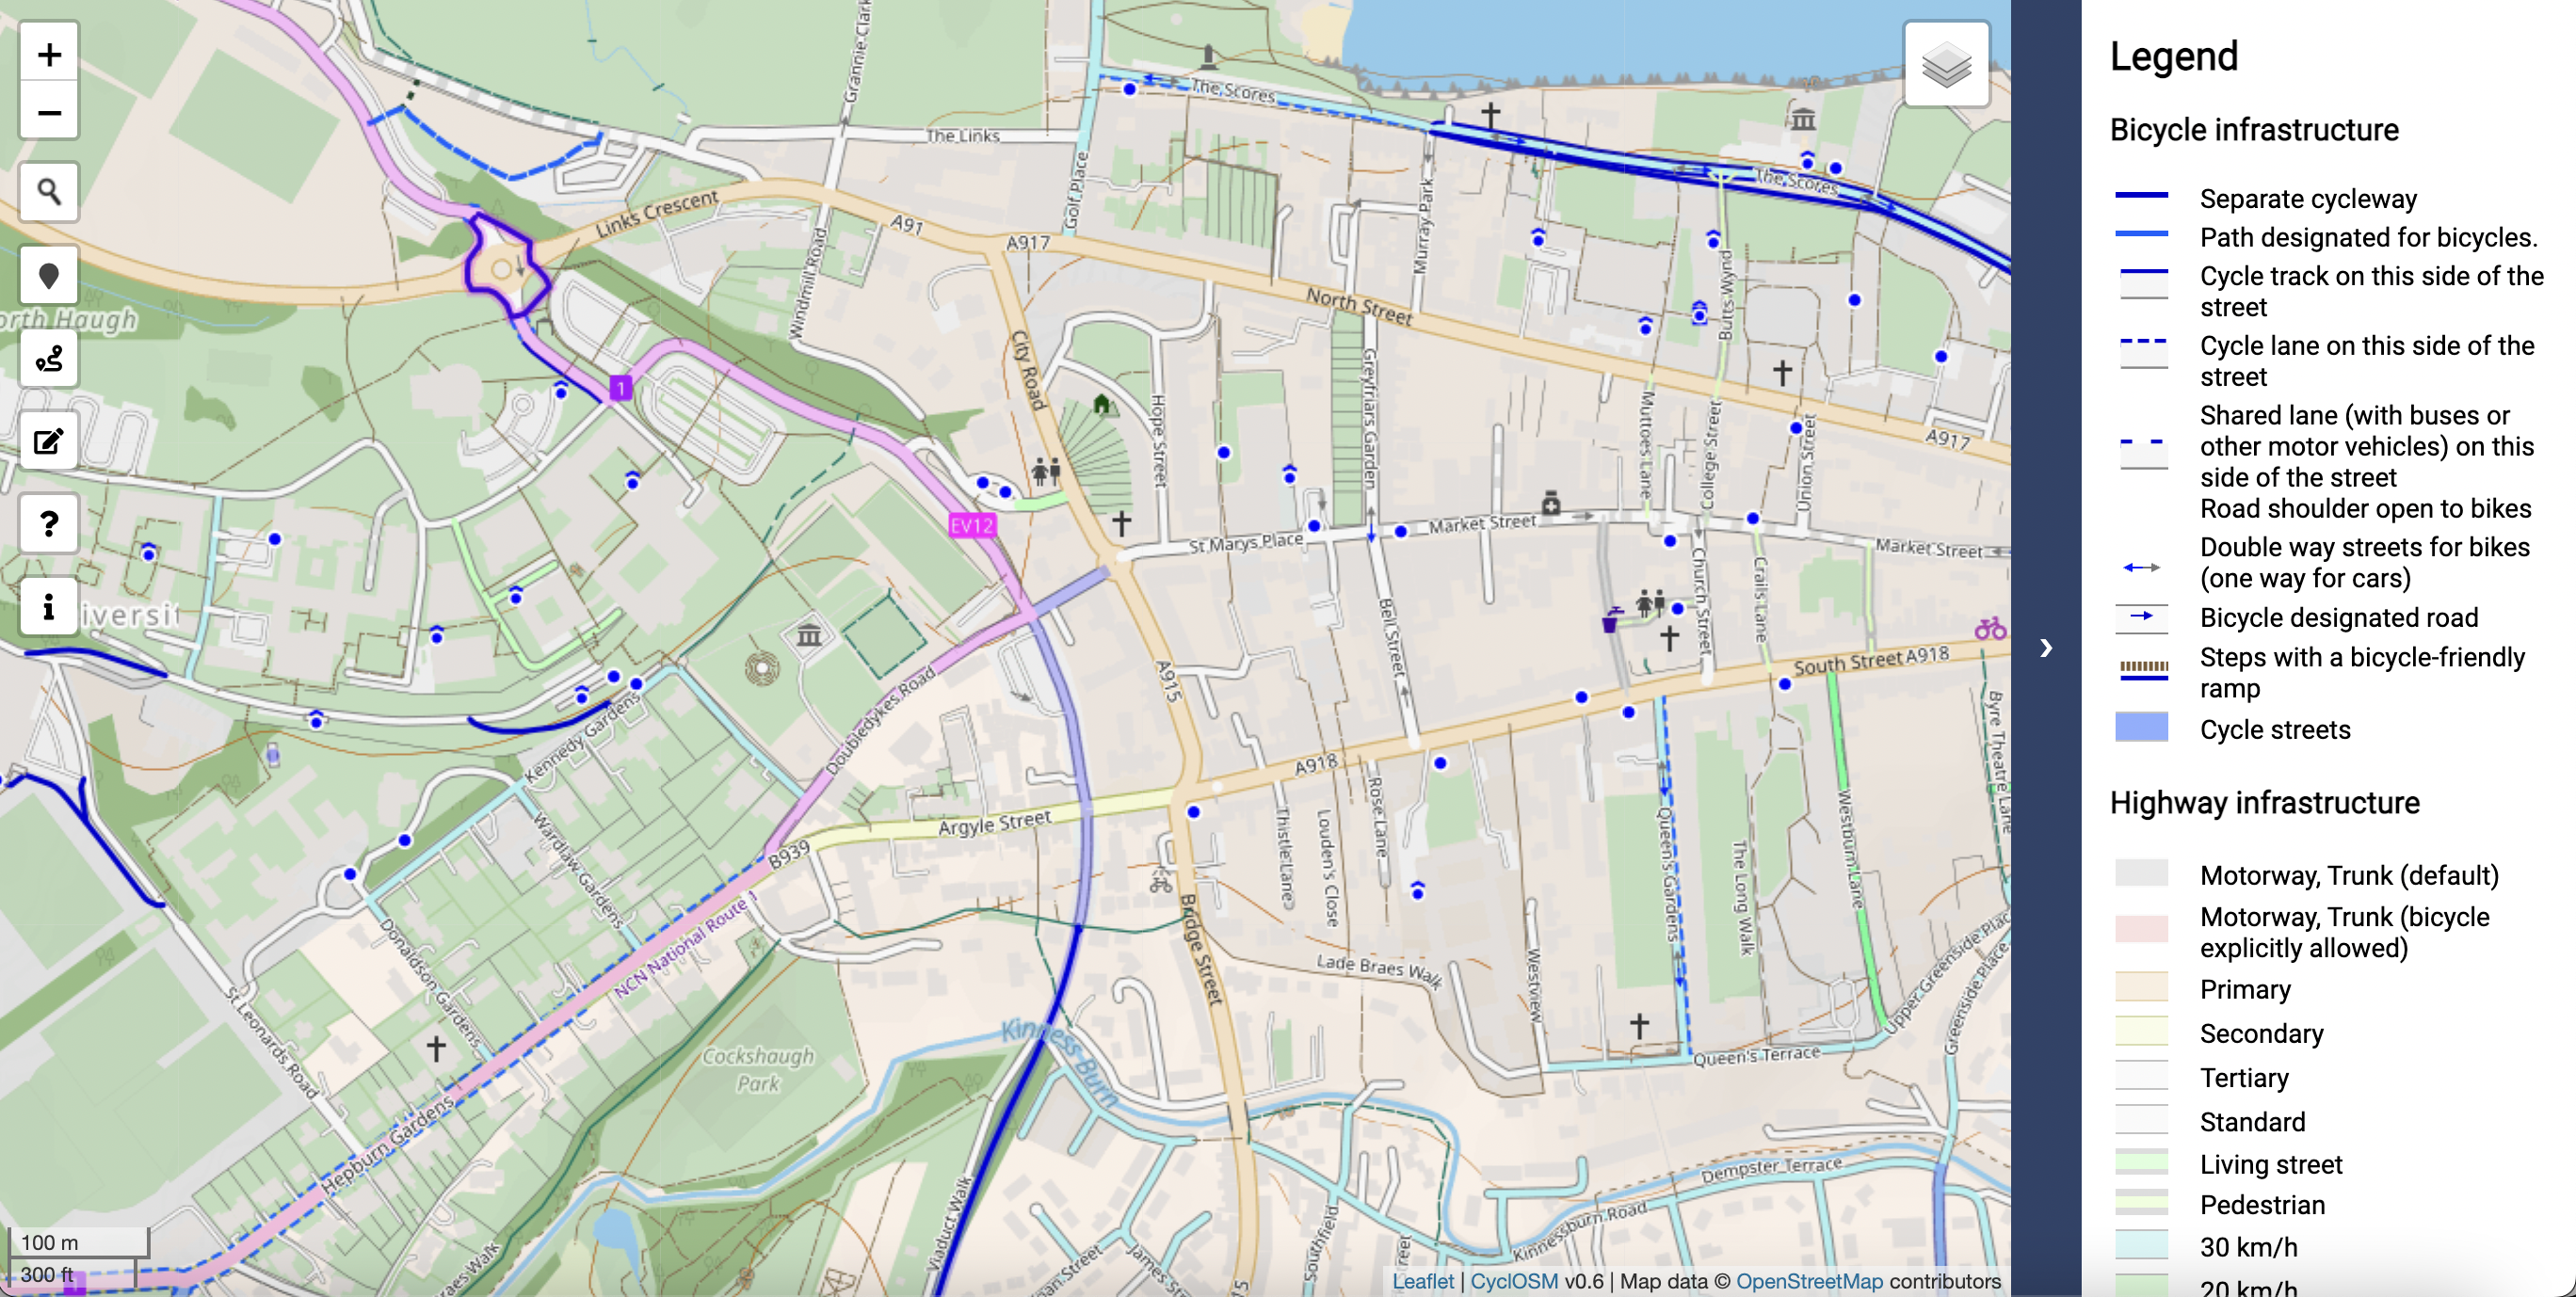
\includegraphics[width=0.8\textwidth,trim={22cm 10cm 0 0},clip]{diss_images/context/osm.png}
\caption{CyclOSM of St Andrews}
\label{fig:osm_sta}
\end{figure}

\begin{figure}[ht!]
\centering
\includegraphics[width=0.8\textwidth,trim={10cm 0 10cm 5cm},clip]{diss_images/context/googlemap.png}
\caption{Google map of St Andrews}
\label{fig:google_sta}
\end{figure}

Figure~\ref{fig:osm_sta} shows the map of St Andrews in CyclOSM~\cite{cycleOSM}, a bicycle map based on OpenStreetMap. It highlights bicycle infrastructure such as cycleways, and it includes information about highways such as speed limits. Ferster et al. \cite{doi:10.1080/15568318.2018.1519746} compared OSM data against municipal open data in six Canadian cities and concluded that OSM data was more extensive and detailed.

There are other maps that can be used to show bike lanes. For example, Google Maps (\url{https://www.google.com/maps}) is a widely used map. More than 1 billion people use it every month~\cite{ethan2019}, and by 2018 it supported 40 languages~\cite{yamagami2018}. It makes use of machine learning techniques to remove fake content and help keep the map accurate~\cite{gupta2023}. It also provides a good user interface. Figure~\ref{fig:google_sta} shows the map of St Andrews in Google Maps in the cycling layer. One advantage that google have over OpenStreetMap is that the map data is not all contributed by volunteers, so it is much easier for them to keep their data consistent.

\begin{figure}[ht!]
    \centering
    \includegraphics[width=0.7\textwidth,trim={0 8cm 5cm 0},clip]{diss_images/context/feature.png}
    \caption{Querying features in OpenStreetMap}
    \label{fig:feature_query}
\end{figure}

\begin{figure}[ht!]
    \centering
    \includegraphics[width=0.7\textwidth,trim={0 5cm 5cm 0},clip]{diss_images/context/cycleway.png}
    \caption{Details of Viaduct Walk}
    \label{fig:cycleway_query}
\end{figure}

One disadvantage of Google Maps is that it is not open data. On the other hand, OpenStreetMap is open data, and it provides much more detailed information regarding bicycle infrastructure. The OpenStreetMap website~\cite{OpenStreetMap} allows users to query features at any point on the map. Figure~\ref{fig:feature_query} shows an example of queried features. Details of each feature can be viewed by clicking the blue text. For example, \textit{Viaduct Walk} is a link to the information page of Viaduct Walk (Figure~\ref{fig:cycleway_query}). It contains a series of tags which specify useful information such as the type of the road, whether pedestrians are allowed and whether it is one-way. It also contains a list of nodes which are on the path. Such information can be helpful for deciding whether a road is cycle-friendly.

\subsection{Overpass API}
OpenStreetMap exposes its data through an API, \textit{Overpass API}~\cite{wiki:overpass}. This API means it is feasible to automate our system. It allows nodes, ways and relations to be queried according to a well-documented query language, \textit{Overpass QL}~\cite{wiki:overpassql}. 

For example, if we want to query nodes for post boxes within a certain area, the query would be
\begin{verbatim}
    node["amenity"="post_box"]({{bbox}});
    out;
\end{verbatim}
where \texttt{bbox} is the bounding box for the area, specified by a 4-tuple \texttt{(south, west, north, east)} in longitude and latitude.

We could also query each OSM element by ID. To get the information associated with Viaduct Walk as shown in Figure~\ref{fig:cycleway_query}, we could use
\begin{verbatim}
    way(151283936);
    out;
\end{verbatim}
where 151283936 is the element ID of Viaduct Walk. This query returns the data in Figure~\ref{fig:query}.

\begin{figure}[ht]
    \centering
    \begin{minipage}[c]{\textwidth}
        \begin{verbatim}
            <way id="151283936">
                <nd ref="297685799"/>
                <nd ref="9097834868"/>
                <nd ref="9356781484"/>
                <nd ref="9356781485"/>
                <nd ref="287216154"/>
                <nd ref="1479980590"/>
                <nd ref="9356781486"/>
                <nd ref="1479980462"/>
                <nd ref="287216155"/>
                <nd ref="985936350"/>
                <nd ref="9356781487"/>
                <nd ref="9356781488"/>
                <nd ref="287216156"/>
                <nd ref="1478202890"/>
                <nd ref="1478202850"/>
                <nd ref="1478203126"/>
                <tag k="foot" v="yes"/>
                <tag k="highway" v="cycleway"/>
                <tag k="lcn" v="yes"/>
                <tag k="name" v="Viaduct Walk"/>
                <tag k="oneway" v="no"/>
                <tag k="surface" v="asphalt"/>
            </way>
        \end{verbatim}
    \end{minipage}
    \caption{Query result of Viaduct Walk}
    \label{fig:query}
\end{figure}

We have access to the list of nodes on Viaduct Walk as well as the tags associated with it. Tags such as \texttt{highway=cycleway} are likely to be helpful in deciding whether an OSM way is cycle-friendly.

\subsection{Applications of graph theory}
In this section, we give an overview of how graph theory has been applied to transportation problems. Erath et al.~\cite{erath2009} studied modern measures of the efficiency of transport metrics where they compared cost in the network against the straight-line distance, and showed that parts of the Swiss road network have reached growth limits, where it is hard to improve them any more owing to spatial limitations.

Derrible and Kennedy~\cite{derrible2011} described the history of graph theory with respect to transportation networks, paying particular note to the development of indicators describing the properties of transportation networks. They highlight the \textit{scale-free} concept from network theory, where in some graphs the probability distribution of the number of connections a node has follows a power law and is not related to the number of edges or vertices in the graph. The process for adding cycle-friendly edges outlined in this project could promote a \textit{scale-free} cycle-friendly network, since we are more likely to add edges to vertices which already have a high number of connections. 

Zargham et al.~\cite{zarghami2020} used spanning trees to quantify network reliability, another measure that may be of relevance to cyclists so that they can be confident of an alternative route should there be any roadworks. They demonstrate an exact measurement of network reliability by looking at the set of all spanning trees in the graph and the probability of no failure for each spanning tree. This could be applied to road networks if we used historical data about roadworks along certain routes to estimate the probability of an edge being open.

\subsection{Applications of Prim's algorithm}
There are many applications of Prim's algorithm. Wang et al.~\cite{wang2018} developed an algorithm based on Prim's algorithm and used it to identify natural disasters in isolated areas. Fitina et al.~\cite{fitina} discussed applying Prim's algorithm in the context of tourism in Papua New Guinea, in order to reduce the expense of travelling between the islands. Iqbal et al.~\cite{iqbal2017} used Prim's algorithm to optimize the planning of fibre optic cables to reduce the costs. We can see that Prim's algorithm is often used to find the most efficient overall routes, and we would like to improve these routes when building new cycling infrastructure. 

\subsection{Software and tools}
Below we discuss some libraries and tools that might be relevant to our project.

\subsubsection*{Overpass API}
\texttt{overpy}~\cite{overpy} is a python wrapper to access the Overpass API. It supports querying with Overpass QL as well as parsing the response data to objects such as nodes and ways. 

\subsubsection*{Graph visualization}
\texttt{Matplotlib}~\cite{Hunter:2007} is a powerful tool for visualizing graphs in python. It was used to display the generated graphs in this project.

\subsubsection*{Graph analysis}
\texttt{NetworkX}~\cite{SciPyProceedings_11} is an open source python library for analysing graphs. It has implementations of standard graph algorithms such as graph traversal and cycle detection. Furthermore, it provides support for graph visualization with \texttt{Matplotlib}. It was used to perform graph analysis in this project.

\texttt{python-igraph}~\cite{igraph} is another useful library for graph manipulation. It also comes with standard graph algorithms and supports graph plotting with either \texttt{Matplotlib} or \texttt{Cairo}~\cite{cairo} which is a graphics library.

\subsubsection*{Version control and backup}
\texttt{Git} was used for version control and the project was pushed to a private \texttt{GitHub} repository regularly so that it can be easily recovered in case of machine failure.

\chapter{Design}\label{chapter:design}
In this chapter, we describe the structure of our system and outline some important design decisions.

\section{System Structure}
The system was divided into three layers: a \textbf{data fetcher} layer, a \textbf{model} layer and a \textbf{graph} layer. The data fetcher makes queries to the Overpass API and stores the street map data returned by the API. The model evaluates cycle-friendliness of the street map data based on certain criteria and uses it to construct nodes and edges. The graph layer builds a graph from the model and analyses the graph to suggest new paths. Figure~\ref{fig:structure} shows the structure of the system. This multi-layer structure also facilitates easier unit testing.

\begin{figure}[ht]
    \centering
    \includegraphics[width=0.5\textwidth]{diss_images/design/multi_layer.png}
    \caption{Structure of the system}
    \label{fig:structure}
\end{figure}

\subsection{Data fetcher layer}
All requests to the Overpass API are carried out by the data fetcher. An example query would be requesting all the ways within an area, specified by a bounding box. The result of the queries are stored in the data fetcher, and it exposes methods that are used by the \textbf{model} layer to select data.

\subsection{Model layer}
The model layer provides logical functions to process the data provided by the data fetcher. For example, given an OSM way, the model can evaluate its cycle-friendliness based on the tags associated with the way. In addition, the model converts the OSM data to a graph structure which consists of nodes and edges. This step is necessary because each OSM way may contain more than two nodes, and most graph libraries such as \texttt{NetworkX} do not support edges with more than two nodes. 

\subsection{Graph layer}
The graph layer constructs a \texttt{NetworkX} graph from nodes and edges provided by the model layer and performs analysis on it. It exposes methods to visualize and modify the graph, as well as to run various shortest path algorithms on the graph. If a framework other than \texttt{NetworkX} was preferred, all that would need to be replaced is the graph layer.

\section{Data Fetcher}
The data fetcher contains the OSM data. This includes all the OSM nodes and ways within the area to be analysed. It should provide access to the relevant information regarding a node or a way. For example, we can store a mapping from node IDs to node objects, and in other layers (model and graph) we can use the lightweight node IDs to represent vertices, and we only access the actual node object when needed. This provides a form of abstraction: the model layer and the graph layer do not need to know the implementation details of OSM nodes and ways; they only need access to some properties such as node positions and way tags, which are provided by the data fetcher.

Ideally, the OSM data returned by any requests can be cached in the data fetcher so that we do not make a new query for every OSM node we are interested in. The data fetcher should also provide some basic error handling, such as when some data is missing.

\section{Model}
The model processes the OSM data from the data fetcher. The main tasks of this layer include:
\begin{itemize}
    \item selecting OSM ways based on their cycle-friendly scores, and
    \item converting OSM ways to vertices and edges to be used by the graph layer
\end{itemize}

The heuristic function to evaluate the cycle-friendliness of an OSM way lies in this layer. For the selection task, we keep a list of OSM ways whose scores are higher than some threshold. To convert OSM ways to a graph, we can process each OSM way in turn, convert OSM nodes to vertices and add edges to connect neighbouring nodes.

For path finding purposes, we would like to construct two graphs: a cycle-friendly graph from cycle-friendly OSM ways, and a city graph from all OSM ways. The logic to convert the OSM ways to a graph is the same; the only difference in the process is the selection of OSM ways. For the city graph, we simply do not perform the selection, or we select all OSM ways. The output of this layer should be nodes and edges of each graph.

There are several ways to represent a graph, using a list of edges or an adjacency list. We decided that the model layer should return an adjacency list, where each node ID is linked to a list of node IDs as its neighbours. This is the most natural way to represent our graph, as we are dealing with neighbouring nodes when processing OSM ways.

\section{Graph}
The graph receives an adjacency list from the model. To plot the graph, we need positions of each node, and this information is available in the data fetcher. The graph layer obtains node positions through the model layer, where the model requests this data from the data fetcher.

On receiving the layout of nodes, the graph layer computes edge lengths according to node positions. All graph analysis happens in this layer, including path finding and component analysis. It should also provide methods to display and save the plots.

\subsection{Path finding strategies} \label{sec:strategies}
In Section \ref{sec:aims}, we mentioned that we would like to suggest the most efficient path to add to the graph to improve the connectedness of the cycling network. However, the definition of the \textit{most efficient} path varies depending on what the user needs the most. It could be that the user only wants to find the shortest path that would connect two big components, or maybe it is more important for the new path to be as central as possible. Four strategies with different priorities were designed to suggest paths.

\subsubsection*{Strategy A: Overall shortest path}
A simple strategy to improve the connectedness of the cycle-friendly subgraph would be to add a path to connect the largest component (region 1) and the second-largest component (region 2). Given the graph of the whole area, we search for the shortest path from any node in region 1 to any node in region 2. Making this path cycle-friendly would connect region 1 and region 2 in the cycle-friendly subgraph and hence improving connectedness.

\subsubsection*{Strategy B: Shortest path via town centre}
One potential issue with strategy A is that the suggested path may be located at the edge of the town, which could be inconvenient for cyclists and its use rate might be low. To address this, strategy B attempts to find the shortest path from the most central node in region 1 to the most central node in region 2, where the most central node in a region is defined to be the node closest to the centre of the town.

\subsubsection*{Strategy C: Shortest path via local centre}
Strategy C works in a similar fashion as strategy B. It searches for the shortest path from the most central node in region 1 to the most central node in region 2. However, the most central node in a region does not depend on the centre of the town. Instead, it is defined to be the node closest to the centre of the region, i.e. the centre of the component.

\subsubsection*{Strategy D: Using existing cycle paths}
In this strategy, we set the path cost for pre-existing cycle paths to be zero. This prioritizes using the pre-existing cycling infrastructure rather than spending money adding paths that are not needed. One effect of this approach is that no matter where in a component we start, any new paths suggested using the shortest path approach will be the same. This is because the cost to move anywhere within a cycle-friendly component would be zero. Hence, this can be considered as an extension of strategy A, with different path costs.

\section{System Configuration}\label{sec:config}
As discussed in Section \ref{sec:aims}, the system should be flexible so that it can be applied to another area. To achieve this, the following attributes were designed to be configurable:

\begin{itemize}
    \item the bounding box of the area
    \item the heuristics to evaluate the cycle-friendliness of an OSM way
    \item the threshold for an OSM way to be considered cycle-friendly
    \item the strategy to find the most efficient way to improve cycle infrastructure
\end{itemize}

There should be a configuration file which is independent of the system code and can be passed to the system as an argument. In the following sections, we would discuss how each attribute can be configured.

\subsection{Area specification}
The area can be specified by two things: the \textit{node ID} of the town or city, and the \textit{bounding box} to run the analysis on. The node ID was required for uniquely identifying a place, and the bounding box was used to limit the data to the region.

\subsection{Cycle-friendly heuristics} \label{sec:cycle_heuristic}
A heuristic function was designed to give a score to an OSM way depending on the tags associated with it to represent how cycle-friendly it is. The score was calculated by
\begin{equation}\label{eq:heuristic}
    h(way) = \frac{\sum_{t\in way.tags} w_t \times s_t}{\sum_{t\in way.tags} w_t}
\end{equation}
where each tag $t$ is a key-value pair, $w_t$ is the weight assigned to tag $t$, $s_t$ is the score gained for tag $t$ to take its value, and $h(way)$ is the score given to the OSM way. This is essentially a weighted average of tag value scores, and both $w_t$ and $s_t$ are configurable. 

Suppose in the configuration file we have two tags, \textit{cycleway} and \textit{smoothness}. We specify that the weight assigned to each tag is
\begin{align*}
    w_{cycleway} &= 1 \\
    w_{smoothness} &= 0.5
\end{align*}

And the score assigned to each tag value is
\begin{align*}
    score(cycleway,\, track) &= 1 \\
    score(cycleway,\, share\_busway) &= 0.6 \\
    score(smoothness,\, excellent) &= 1 \\
    score(smoothness,\, intermediate) &= 0.4
\end{align*}

Now suppose we have an OSM way with the following tags:
\[cycleway=track,\quad smoothness=intermediate\]

The heuristic function should return
\begin{align*}
    h(way) &= \frac{1\times 1 + 0.5\times 0.4}{1 + 0.5} \\
    &= 0.8
\end{align*}

Tags which do not appear in the configuration file are considered unimportant and have zero weight.

\subsection{Cycle-friendly threshold}
The heuristic function assigns a cycle-friendly score to each OSM way, and we would like to make the binary decision of whether a way should be classified as cycle-friendly based on its score. We could define a threshold in the configuration file, and consider a way to be cycle-friendly only if it gives a score higher than the threshold. The choice of the threshold value is important. If it is set too high, not many ways will be selected; if it is set too low, not much filtering will happen and the resulting graph will not give much useful information.

\subsection{Strategies}
User should be able to specify which strategies they prefer to use, as discussed in Section~\ref{sec:strategies}. The default is to run all strategies on the graph.

\chapter{Implementation}\label{chapter:impl}
This chapter focuses on the implementation of our system. Sections~\ref{sec:data fetcher impl}, \ref{sec:model impl} and \ref{sec:graph impl} outline the implementation of each layer. Section~\ref{sec:client} discusses the terminal client for the system. Testing was carried out and explained in Section~\ref{sec:testing}.

\section{Data Fetcher}\label{sec:data fetcher impl}
All queries to the Overpass API were made in the data fetcher layer. Given the bounding box of an area to be analysed, we are interested in all the nodes and ways within this area. This data could be fetched using the query
\begin{verbatim}
    nwr(south, west, north, east); out;
\end{verbatim}
where the tuple \texttt{(south, west, north, east)} specifies the bounding box, and \texttt{nwr} stands for nodes, ways and relations.

We used \texttt{overpy} to perform the query and the result was cached in a \texttt{Result} object. The following was provided to the model layer:
\begin{enumerate}
    \item All the OSM ways within a given area
    \item A method to fetch all the nodes on a given OSM way
    \item A method to get the location of a given OSM node, in longitude and latitude
\end{enumerate}

The model needs access to all the OSM ways as well as all the nodes on each way so that it can analyse the cycle-friendliness of ways and convert ways to nodes and edges. The location of each node is helpful when plotting the graph.

The OSM ways in the area were stored in \texttt{Result.ways}, which is a list of \texttt{Way} objects. To get all the nodes on a given way, the \texttt{Way} object provides a \texttt{get\_nodes} method. The longitude and latitude of a node can be accessed by \texttt{Node.lon} and \texttt{Node.lat}.

It should be noted that when querying data within a bounding box, the returned \texttt{Way} may not be completely inside the bounding box, since Overpass API would return all the ways including the ones that are only partly inside the boundary. This means that when we fetch all the nodes on a given way, some nodes may be outside the bounding box. To keep the graph clean and focused, we would like to disregard nodes that are outside the boundary.

\section{Model}\label{sec:model impl}
The model layer handles the filtering of OSM ways. Since we were interested in the cycle-friendly subgraph, we implemented a heuristic function that gives a cycle-friendly score to each way by analysing the tags associated with it, as defined in Equation \ref{eq:heuristic}.

Two data classes, \texttt{Tag} and \texttt{WeightedTags}, were created to store the weighting of the tags. \texttt{Tag} has two attributes:
\begin{itemize}
    \item \texttt{weight}, which is a float representing the tag weight
    \item \texttt{values}, which maps each tag value to a score
\end{itemize}

On the other hand, \texttt{WeightedTags} stores a mapping from a tag key to a \texttt{Tag}. It also provides a method, \texttt{weight\_sum}, which calculates the sum of weight for all the tags. These data classes facilitated the implementation of Equation \ref{eq:heuristic}. With the score function, we could select cycle-friendly ways based on a given threshold.

The next step was to convert OSM ways to vertices and edges. Since each OSM way could consist of more than two nodes, a simple method to convert it into edges would be breaking the way at each intermediate node. For example, consider an OSM way represented by
\[A - B - C - D\]
Since each way is an ordered list of nodes, we could represent it using three edges:
\[A - B, B - C, C - D\]

The number of vertices and edges we obtained using this approach would greatly depend on the size of the area. To simplify the graph, we would like to keep nodes that are either at the beginning or the end of a way, or if they appear on more than one way. We introduced a \textit{link counter} to keep track of the number of links each node has. This is done by going through all the ways and incrementing the counter for each node on the way.

Then, we can use the \textit{link counter} to convert OSM ways into edges, represented by an adjacency list. For each OSM way, we look at every intermediate node, i.e. any node that is not at the beginning nor the end of the way. If a node has more than one link, we keep the node and break the way at this node; otherwise, we ignore the node. The pseudocode for this algorithm is demonstrated in Algorithm~\ref{alg:adj}.

\begin{algorithm}
\caption{An algorithm to convert hyperedges to an adjacency list}\label{alg:adj}
\begin{algorithmic}
\Require $hyperEdges, counter$
\Ensure $adj$
\State $adj\gets \emptyset$
\For{$e$ \textbf{in} $hyperEdges$}
    \State $currentPointer\gets 0$
    \State $currentNode\gets e[currentPointer]$
    \State $nextPointer \gets currentPointer + 1$
    \While{$nextPointer < length(e)$}
        \State $nextNode\gets e[nextPointer]$
        \If{$counter[nextNode] > 1$ \textbf{or} $nextPointer = length(e)-1$}
            \If{$currentNode \neq nextNode$}
                \State $neighbours\gets$ empty list
                \If{$currentNode$ \textbf{in} $adj$}
                    \State $neighbours\gets adj[currentNode]$
                \EndIf
                \State add $nextNode$ to $neighbours$
                \State $adj[currentNode]\gets neighbours$
                \State $currentPointer\gets nextPointer$
                \State $nextPointer\gets currentPointer + 1$
            \EndIf
        \Else
            \State $nextPointer\gets nextPointer + 1$
        \EndIf
    \EndWhile
\EndFor
\end{algorithmic}
\end{algorithm}

\section{Graph}\label{sec:graph impl}
In the graph layer, we construct a graph from vertices and edges provided by the model layer. Two graphs were created: a graph that only consists of cycle-friendly edges, known as the \textit{cycle-friendly graph}, and a graph which consists of all edges regardless of their cycle-friendliness, known as the \textit{city graph}. Our goal was to find a path in the city graph that if it were to be made cycle-friendly, the connectedness of the cycle-friendly graph would improve the most.

\subsection{Choice of graph libraries}
Two graph libraries, \texttt{NetworkX} and \texttt{python-igraph}, were experimented with during the implementation. We discovered that \texttt{NetworkX} produced better plots using \texttt{Matplotlib} than \texttt{python-igraph} did. Figure~\ref{fig:igraph} and \ref{fig:networkx} shows a plot produced by \texttt{python-igraph} and \texttt{NetworkX} respectively. We can see that the \texttt{igraph} plot is much more compact, and it is very difficult to distinguish nodes next to each other. On the other hand, \texttt{NetworkX} provides better colouring settings and the resulting plot is tidier. Therefore, \texttt{NetworkX} was the main library used in the graph layer.

\begin{figure}[ht]
    \centering
    \includegraphics[width=0.7\textwidth]{diss_images/impl/igraph.png}
    \caption{A plot of St Andrews produced by \texttt{python-igraph}}
    \label{fig:igraph}
\end{figure}

\begin{figure}[ht]
    \centering
    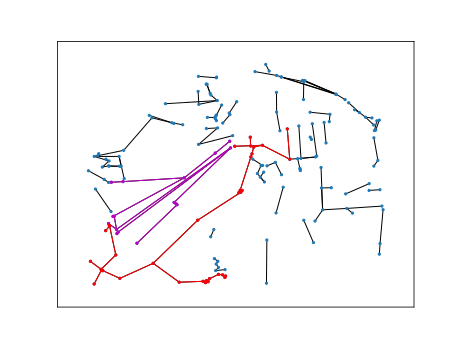
\includegraphics[width=0.7\textwidth,trim={2.5cm 1.5cm 1.7cm 1.7cm},clip]{diss_images/impl/networkx.png}
    \caption{A plot of St Andrews produced by \texttt{NetworkX}}
    \label{fig:networkx}
\end{figure}

\subsection{Plotting}
We obtained nodes and edges from the OSM data in the model layer, and we would like to plot the graph to see how well it represents the St Andrews area. To achieve this, each node must be given a position. Since we had access to the longitude and latitude of a node, we created a mapping from node ID to node coordinates, and this was used as a position attribute assigned to each node. Figure~\ref{fig:graph layout} shows the plot of the cycle-friendly graph overlaying the OpenStreetMap of St Andrews.

\begin{figure}[ht]
    \centering
    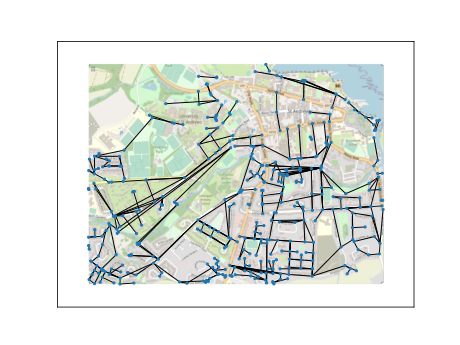
\includegraphics[width=0.7\textwidth]{diss_images/impl/graph_layout.png}
    \caption{The cycle-friendly graph overlaying the OpenStreetMap}
    \label{fig:graph layout}
\end{figure}

\subsection{Geometric edges}
A closer look at the constructed graph reveals a problem. Figure~\ref{fig:close before} shows part of the cycle-friendly graph, where the red region is the largest connected component in the graph. We can see that the right most part of the red region appears to be connected to the edge next to it, but they were actually not connected in the graph. Figure~\ref{fig:osm close} shows the corresponding part in OpenStreetMap. Although Lade Braes Walk (vertical red dotted line) and Queen's Terrace (horizontal white solid line) do not share any nodes on OSM, it seems like they do have an intersection, so they should be considered as connected. In addition, Figure~\ref{fig:google close} shows the Google Maps street view of Queen's Terrace, where Lade Braes Walk is clearly accessible. These connections do not always exist on OpenStreetMap because its primary purpose is to render graphical maps where the geographical connections are obvious, so this aspect of data validation is not the highest priority for the mappers.

\begin{figure}[ht]
    \centering
    \begin{subfigure}[ht]{0.45\textwidth}
        \centering
        \includegraphics[width=\textwidth]{diss_images/impl/close_before.png}
        \caption{Before adding geometric edges}
        \label{fig:close before}
    \end{subfigure}
    \hfill
    \begin{subfigure}[ht]{0.45\textwidth}
        \centering
        \includegraphics[width=\textwidth]{diss_images/impl/close_after.png}
        \caption{After adding geometric edges}
        \label{fig:close after}
    \end{subfigure}
       \caption{Part of the cycle-friendly graph}
       \label{fig:close example}
\end{figure}

There are many other examples in our constructed graph where nodes are very close to each other but disconnected, even though in real life it is possible for a cyclist to move from one node to another. To address this, for every pair of nodes that are geographically close to each other, we added an edge to connect them. Conveniently, \texttt{NetworkX} provides a method called \texttt{geometric\_edges} which computes the edge list of node pairs within a certain radius of each other. This radius is configurable in the configuration file. Figure~\ref{fig:close after} shows the graph after connecting close nodes, with radius set to 0.0005. The red region which represents the largest component is now larger, connecting nodes and edges that are nearby.

\begin{figure}[ht]
    \centering
    \includegraphics[width=0.7\textwidth]{diss_images/impl/osm_close.png}
    \caption{The corresponding part of Figure~\ref{fig:close example} in OpenStreetMap}
    \label{fig:osm close}
\end{figure}

\begin{figure}[ht]
    \centering
    \includegraphics[width=0.7\textwidth]{diss_images/impl/googlemap_cross.png}
    \caption{Google Maps street view of Queen's Terrace}
    \label{fig:google close}
\end{figure}

\subsection{Connected components}
In order to identify isolated islands in the cycle-friendly graph, we would like to analyse the connected components in the graph. \texttt{NetworkX} provides methods to find connected components, and we are interested in connecting the largest component with the second-largest component. There are a few possible definitions of \textit{the largest} component; it could be the component that contains the most nodes, the most edges, the largest geographical area or one with the largest total edge length. We decided to use edge length as the metric because that metric is an exact measurement of the cycle-friendly infrastructure, and doesn't suffer if there is a variation in the density of nodes between components.

In order to calculate the total edge length for each component, we first compute the total length of all the edges inside the component. Then, we sort the connected components using this criterion and identify the two largest component, as demonstrated in Figure~\ref{fig:component}.

Another approach we considered was to measure the geographical area enclosed by the component, as this may correlate better with the number of people who can utilise the cycling infrastructure. This was challenging to measure accurately because the formulae for calculating the area of an irregular polygon assume that its boundary is known. However, we have a large collection of nodes, and it is difficult to distinguish which nodes are on the boundary and which are not. One possible way to find the boundary is to take the extreme compass points, i.e. the nodes with the greatest and least longitude and latitude. The problem with this approach is that we may not always end up with more than two nodes, for example, when the north-most node is also the east-most node, and the south-most node is also the west-most node. In this case, the nodes would form a line which has no area.

\begin{figure}[ht]
    \centering
    \includegraphics[width=0.8\textwidth,trim={2.5cm 1.5cm 1.7cm 1.7cm},clip]{diss_images/impl/components.png}
    \caption{Connected components in the cycle-friendly graph}
    \label{fig:component}
\end{figure}

\subsection{Weighted graph}\label{sec:weighted}
Our strategies involve running the shortest path algorithm on the graph. This shortest path should reflect on the actual length of the path in the map, which means we have to assign weights to edges. This could be achieved easily if we were provided with the length of each OSM way, but this data is not available on the Overpass API. Hence, we would like to estimate the length of an edge based on node coordinates. Given two nodes, $u$ and $v$, and their coordinates, $u = (u_0, u_1)$ and $v = (v_0, v_1)$, where $u_0, v_0$ is the latitude and $u_1, v_1$ is the longitude, we can compute the geodesic distance between the nodes using \texttt{geopy}~\cite{geopy}, a python package for geocoding. This distance could be used as the weight of the edge $uv$.

\subsection{Strategies}
Recall that we discussed four strategies in Section~\ref{sec:strategies}. All these strategies involve finding the shortest path. \texttt{NetworkX} provides an implementation of Dijkstra's algorithm, and this was utilised differently for each strategy. 

\subsubsection*{Strategy A: Overall shortest path}
To find the overall shortest path between two regions, we ran Dijkstra's algorithm from every node in region 1 to every node in region 2. For each path found, we kept track of the length of the path as well as the path itself, in the form of a list of nodes on the path. Each time a shorter path was found, we replaced the stored path with the new shorter path. Eventually, we ended up with the overall shortest path between the two regions.

\subsubsection*{Strategy B: Shortest path via town centre}
In OpenStreetMap, there is a node representing the centre of St Andrews. Since OSM nodes have coordinates, we used this to find the nearest node to the centre of St Andrews in each region. The distance from a node to the centre was calculated using the geodesic distance. After finding the most central node for each region, we used Dijkstra's algorithm to compute the shortest path between these nodes.

\subsubsection*{Strategy C: Shortest path via local centre}
In strategy C, we find the nodes that are central within each region. A method called \texttt{NetworkX.centre} was used to obtain the set of central nodes of a graph, where the maximal distance from the central nodes to other nodes in the graph is minimized. We could construct a subgraph for each region and find the central nodes. For simplicity, we took the first returned node as the centre of the region. After that, we ran Dijkstra's algorithm from the central node in region 1 to the central node in region 2.

\subsubsection*{Strategy D: Using existing cycle paths}
In strategy D, we set all pre-existing cycle paths to have zero cost. For every edge in the cycle-friendly graph, we set its edge weight to be zero in the unfiltered graph. Then, we run Dijkstra's algorithm in the same manner as strategy A, in order to obtain the shortest path.

\section{Terminal Client}\label{sec:client}
A script called \texttt{main.py} was written to provide an entry point to the system, which enables the automation of the cycle infrastructure analysis. The \texttt{argparse} module was used to write the command line interface, and our system allows two arguments:
\begin{itemize}
    \item \texttt{--config}, which specifies the path to the configuration file
    \item \texttt{--save}, which specifies the directory to save the generated graphs
\end{itemize}

A default configuration file was provided in Appendix~\ref{app:config}, but a user-defined configuration file can be passed to the system. This allows users to run the system on multiple configurations and compare the results easily, without the need to modify a single configuration file repeatedly. Users can also specify where to save the generated plots.

\section{Testing Approach}\label{sec:testing}
As our system was implemented in a multi-layer architecture, we were able to test each layer independently. The following python libraries were used for testing:
\begin{itemize}
    \item \texttt{unittest}~\cite{unittest}, which is a python framework for unit testing
    \item \texttt{unittest.mock}~\cite{unittest:mock}, which is used to mock objects
    \item \texttt{coverage}~\cite{coverage}, which is a tool for measuring test coverage
\end{itemize}

The testing results are shown in Appendix~\ref{app:test}. In the following sections, we give an overview of how unit testing was carried out for each layer.

\subsection{Data fetcher}
Most methods provided in the data fetcher are attribute getters, so unit tests were written to verify the correct attribute was returned by each method. We used mock OSM ways and nodes for testing so that we could set their attributes without the need to make a request to the Overpass API. In addition, the \texttt{patch} decorator was used to create a mock object of the Overpass API, so that the unit tests would not be dependent on the Overpass API server.

\subsection{Model}
Unit tests were written for each method in model, with edge cases considered where applicable. A mock data fetcher was used when creating the model so that we could focus on the behaviour of model without being affected by the data fetcher. Similar to data fetcher tests, we used mock OSM ways when testing methods such as \texttt{eval\_way}, the heuristic function to give a score to an OSM way. This allows us to configure the tags associated with each way easily, and the method was tested with many configurations.

\subsection{Graph}
In the graph layer, most of the code were written to display a plot or were direct wrappers of functions in the \texttt{NetworkX} library. It was difficult to write unit tests for graph visualization, and widely-used libraries such as \texttt{NetworkX} are likely to be well-tested. Hence, tests were only written for auxiliary methods in this layer which do not involve plotting or graph analysis in \texttt{NetworkX}.

\chapter{Evaluation}\label{chapter:eval}
In this chapter, we reflect on the goals and objectives of this project. We will look at the plots generated by our system and discuss the effectiveness of the suggested paths.

\section{Configuration}
As discussed in the design and implementation chapters, the system is designed in such a way that the choice of which tags contribute to the cycle-friendly score are the responsibility of the user. A default configuration file (Appendix~\ref{app:config}) was created using the legend and documentation of CyclOSM~\cite{cycleOSM} as inspiration. CyclOSM uses OpenStreetMap data to highlight cycling infrastructure. Similarly to this project, it utilises the tags of ways, so it is a relatively complete reference for the most important tags to be considered. As mentioned in the context survey, one difficulty with OpenStreetMap is that since different groups of mappers have their own conventions, there are a wide variety of tag-value mappings that represent the same things. As a consequence, CyclOSM does not cover every relevant combination of tags. The extensible configuration means that a local town planner could adapt the system to suit the conventions of the local area.

\section{Cycle-friendly Graph and CyclOSM}\label{sec:eval_osm}
We compared the cycle-friendly graph which was generated by our system against CyclOSM~\cite{cycleOSM}. Figure~\ref{fig:cyclosm st andrews} shows the map of St Andrews in CyclOSM, and the map legend is shown in Figure~\ref{fig:cyclosm legend}.

\begin{figure}[ht!]
    \centering
    \includegraphics[width=0.9\textwidth]{diss_images/eval/cyclosm_st_andrews.png}
    \caption{CyclOSM of St Andrews}
    \label{fig:cyclosm st andrews}
\end{figure}

\begin{figure}[ht!]
    \centering
    \includegraphics[width=0.3\textwidth]{diss_images/eval/cyclosm_legend.png}
    \caption{CyclOSM legend of bicycle infrastructure}
    \label{fig:cyclosm legend}
\end{figure}

\begin{figure}[ht]
    \centering
    \includegraphics[width=0.7\textwidth,trim={1cm 1cm 1cm 1cm},clip]{diss_images/eval/overlay_st_andrews.png}
    \caption{The cycle-friendly graph overlaying the CyclOSM (St Andrews)}
    \label{fig:overlay st andrews}
\end{figure}

\begin{figure}[ht!]
    \centering
    \begin{subfigure}[ht]{0.65\textwidth}
        \centering
        \includegraphics[width=\textwidth]{diss_images/eval/cycle_friendly_old.png}
        \caption{Before the configuration was modified}
        \label{fig:cycle friendly graph old}
    \end{subfigure}
    \hfill
    \begin{subfigure}[ht]{0.52\textwidth}
        \centering
        \includegraphics[width=\textwidth]{diss_images/eval/cycle_friendly_new.png}
        \caption{After the configuration was modified}
        \label{fig:cycle friendly graph new}
    \end{subfigure}
       \caption{The cycle-friendly graph generated by our system}
       \label{fig:cycle friendly graphs}
\end{figure}

The cycle-friendly graph produced by our system using the default configuration is shown in Figure~\ref{fig:cycle friendly graph new}. An earlier produced graph is displayed in Figure~\ref{fig:cycle friendly graph old}. Upon a closer look at some of the paths we discovered an omission in the CyclOSM view. There are a few streets which have a cycle path where the value for the \texttt{cycleway} tag is \texttt{opposite}, however this value is not considered by CyclOSM. Therefore, this tag was added to the default configuration file, and the more complete cycle-friendly graph was produced in Figure~\ref{fig:cycle friendly graph new}.

Figure~\ref{fig:overlay st andrews} shows the cycle-friendly graph overlaying the CyclOSM of St Andrews. We can see that ways with a separate cycle way and paths designated for bicycles are identified in our plot. On the other hand, the busy main roads such as \textit{North Street} and \textit{South Street} do not appear, which is sensible as they are not very safe to cycle on. 

We also identified some additional cycle-friendly paths, which fall into two categories: \begin{enumerate}
    \item Roads that have a cycle path but were not highlighted by CyclOSM for the reasons discussed earlier, such as \textit{Greyfriars Garden}.
    \item Roads that do not have a cycle path, but which our heuristic deemed cycle-friendly, such as \textit{Bell Street}. In this case it is a small tertiary road, so it would likely be acceptable for most cyclists to cycle through there.
\end{enumerate}

Since \textit{Bell Street} connects to \textit{Greyfriars Garden}, it would seem reasonable for cyclists to use this route to go from \textit{South Street} to \textit{North Street} using the existing cycling infrastructure. This route is not highlighted in CyclOSM, but it is considered cycle-friendly in our plot. Note that one limitation of our system is that we don't consider direction - \textit{Bell Street} is one way for cyclists as well as cars, so it would not be so easy to use this route to go from \textit{North Street} to \textit{South Street}.

\section{Connectivity Analysis}\label{sec:connectivity}
We applied the automated process to analyse the cycling infrastructure in St Andrews. In the following sections, we will discuss the results from graph analysis.

\subsection{Components}\label{sec:components}
Our process has identified 15 components in the St Andrews cycle-friendly graph. The components are highlighted in Figure~\ref{fig:components st andrews}. We have one large component, and lots of smaller components. The empty space at the north of the graph comprises the centre of St Andrews, while the filled-in part to the south and west comprises the bulk of the quieter residential areas and the university. This suggests that it is hard to cycle around the centre of St Andrews, but easy to cycle around the residential neighbourhoods and the university. Therefore, at a glance it might make sense for the town planners to focus on improving cycling infrastructure in the town centre. Since the second largest cycle-friendly component is along the north shore, our system will be likely to suggest paths that will connect these components through the town centre.

\begin{figure}[ht]
    \centering
    \includesvg[width=0.9\textwidth]{diss_images/images_st_andrews/st_andrews_components.svg}
    \caption{The components in the cycle-friendly graph of St Andrews}
    \label{fig:components st andrews}
\end{figure}

\subsection{Suggested paths}\label{sec:paths}
The cycle path additions suggested by our system are highlighted in yellow in Figure~\ref{fig:path st andrews}. As might be expected from the initial conditions given to each approach, strategy A chose the shortest connection along the east edge, utilizing North Castle Street. Strategy B chose a route through the centre of St Andrews, and strategy C connected the University Area through to the northern shore. These results highlight the trade-offs inherent to town planning. Strategy A might be the cheapest, but it won't benefit a large number of people, while strategies B and C each favour different groups. It would benefit students the most to improve cycling connections from the university to the centre, whereas normal residents would greatly benefit from a less dangerous approach into town. Strategy D gave the same result as strategy A in this case, as making use of existing cycle paths did not result in a lower cost path. Our system can give town planners concrete suggestions of routes they could plan, and they can select different strategies to use based on their priorities for improvements.

% path st andrews
\begin{figure}[ht]
    \centering
    \begin{subfigure}[ht]{0.47\textwidth}
        \centering
        \includesvg[width=\textwidth]{diss_images/images_st_andrews/st_andrews_path_overall.svg}
        \caption{Strategy A (overall)}
        \label{fig:overall st andrews}
    \end{subfigure}
    \hfill
    \begin{subfigure}[ht]{0.47\textwidth}
        \centering
        \includesvg[width=\textwidth]{diss_images/images_st_andrews/st_andrews_path_town_centre.svg}
        \caption{Strategy B (town centre)}
        \label{fig:centre st andrews}
    \end{subfigure}
    \hfill
    \begin{subfigure}[ht]{0.47\textwidth}
        \centering
        \includesvg[width=\textwidth]{diss_images/images_st_andrews/st_andrews_path_local_centre.svg}
        \caption{Strategy C (local centre)}
        \label{fig:local st andrews}
    \end{subfigure}
    \hfill
    \begin{subfigure}[ht]{0.47\textwidth}
        \centering
        \includesvg[width=\textwidth]{diss_images/images_st_andrews/st_andrews_path_existing.svg}
        \caption{Strategy D (existing)}
        \label{fig:existing st andrews}
    \end{subfigure}
       \caption{Path to improve the cycling infrastructure in St Andrews}
       \label{fig:path st andrews}
\end{figure}

\subsection{Graph metrics}\label{sec:metrics}
As mentioned in the context survey, a common metric of connectedness of a graph is \textit{k-connectivity}. This specifies the minimum number of edges or nodes that could be removed in order for a graph to no longer be connected. The higher the k-connectivity, the more connected the graph is. The connectivity of the original graph of St Andrews is 1, before we do the cycle-friendly processing. This is likely because there are some nodes in dead ends where there is only one route to access them, so removing that one edge will make the graph not connected. Once we apply the cycle-friendly heuristic, the connectivity of the graph becomes 0, because the cycle-friendly graph is not connected and has many components. This suggests that k-connectivity may not be the best measure of connectedness of the cycle-friendly graph.

A related measure is called \textit{average node connectivity}. This may be a better metric than k-connectivity because it is not as affected by individual cases and works even when the graph is not completely connected. We consider, for each pair of nodes, the minimum number of edges that could be removed in order for the nodes to not have a connecting path. We then take the average node connectivity to be the mean value of this metric. It is infeasible to run this algorithm on the original graph because there are too many nodes and the algorithm scales quadratically. However, it is feasible to run this on the cycle-friendly graph.

The average node connectivity of the cycle-friendly graph was 0.947, before we add any new paths to it. This is less than one because, if nodes are in different components, no edges need to be removed to make them disconnected, as they are already disconnected. After connecting the two largest components using any of the four strategies, the average node connectivity increased to 0.999. The same value was given by each strategy, because we were only adding one path to connect the same components. It would be interesting to see if we would see greater improvements in average node connectivity when we added a new region, or if it is better to improve connections within the largest cycle-friendly region. This will likely depend on the characteristics of the graph concerned, so it may vary by each geographical area's cycling infrastructure.

% avg st andrews
\begin{table}[ht]
    \centering
    \begin{tabular}{|c|c|}
        \hline
        Graph & Average shortest path length \\
        \hline
        Unmodified & 4.156 \\
        Strategy A & 3.744 \\
        Strategy B & 3.739 \\
        Strategy C & 3.730 \\
        Strategy D & 3.744 \\
        \hline
    \end{tabular}
    \caption{Comparison of average shortest path length - St Andrews}
    \label{tab:avg st andrews}
\end{table}

Another useful graph metric is the \textit{average shortest path length} of a graph. This calculates the shortest path between each pair of nodes, and takes the mean value of the distance of these paths. The smaller this number, the easier it would be to get from one place to another. The metric in its purest form does not directly apply to a disconnected graph, since not all pairs of nodes will have a path between them. To get around this, we assigned a high constant value to be the cost of commuting between two disconnected nodes. Table~\ref{tab:avg st andrews} shows the value of this metric for the unmodified cycle-friendly graph as well as for the graph modified by each of the strategies.

Since strategy A and D produced the same path, the values for these two strategies are in the same. We can see that strategy C made the biggest difference to average path length, which makes sense because improving the connectivity of the most central node in a region should make a bigger effect on the majority of nodes than improving the connectivity of a node on the outskirts, which is what strategy A did.

\section{Application to Other Areas}
In order to evaluate the scalability of our approach, we have applied the automated process to two other cities: Dundee in Scotland and Houten in the Netherlands. Dundee was chosen because it is nearby St Andrews, and it is much larger than St Andrews, so we might get multiple similarly sized regions rather than one big component. Houten was chosen because it is of a similar size to St Andrews, but has grown much in recent decades. It has been the subject of urban planning designed to promote bicycle usage over driving.

\subsection{Dundee}\label{sec:dundee}
We can see in Figure~\ref{fig:components dundee} that Dundee has many more disconnected components than St Andrews did, and the distribution of the size is much more even. Figure~\ref{fig:overlay dundee} shows the cycle-friendly map overlaying the CyclOSM of Dundee. We can see that there are cycle-friendly clusters around the centres of activity in the city, such as Ninewells Hospital (southwest of the map), the city centre and waterfront (by the river), and the Hilltown (roughly in the centre of the map).

% component + overlay dundee
\begin{figure}[ht!]
    \begin{subfigure}{\textwidth}
        \centering
        \adjustbox{trim=1cm 1cm 1cm 1cm, clip} {
            \includesvg[width=0.9\textwidth]{diss_images/images_dundee/dundee_components.svg}
        }
        \caption{The components in the cycle-friendly graph of Dundee}
        \label{fig:components dundee}
    \end{subfigure}
    \hfill
    \begin{subfigure}{\textwidth}
        \centering
        \includegraphics[width=0.7\textwidth,trim={1cm 1cm 1cm 1cm},clip]{diss_images/eval/overlay_dundee.png}
        \caption{The cycle-friendly graph overlaying the CyclOSM (Dundee)}
        \label{fig:overlay dundee}
    \end{subfigure}
    \caption{The cycle-friendly graph of Dundee}
\end{figure}

The suggested paths are shown in Figure~\ref{fig:path dundee}. Our system suggests that the Ninewells Hospital area and the city centre should be the priority for connecting. This is in fact a project that Dundee City Council are undertaking~\cite{robertson:dundee}. The proposed routes from our system are more direct than those proposed by Dundee City Council, which is likely because we didn't take into account changes in elevation, since our suggested routes go through the Balgay Hill area.

% path Dundee
\begin{figure}[ht]
    \centering
    \begin{subfigure}[ht]{0.47\textwidth}
        \centering
        \includesvg[width=\textwidth]{diss_images/images_dundee/dundee_path_overall.svg}
        \caption{Strategy A (overall)}
        \label{fig:overall dundee}
    \end{subfigure}
    \hfill
    \begin{subfigure}[ht]{0.47\textwidth}
        \centering
        \includesvg[width=\textwidth]{diss_images/images_dundee/dundee_path_town_centre.svg}
        \caption{Strategy B (town centre)}
        \label{fig:centre dundee}
    \end{subfigure}
    \hfill
    \begin{subfigure}[ht]{0.47\textwidth}
        \centering
        \includesvg[width=\textwidth]{diss_images/images_dundee/dundee_path_local_centre.svg}
        \caption{Strategy C (local centre)}
        \label{fig:local dundee}
    \end{subfigure}
    \hfill
    \begin{subfigure}[ht]{0.47\textwidth}
        \centering
        \includesvg[width=\textwidth]{diss_images/images_dundee/dundee_path_existing.svg}
        \caption{Strategy D (existing)}
        \label{fig:existing dundee}
    \end{subfigure}
       \caption{Path to improve the cycling infrastructure in Dundee}
       \label{fig:path dundee}
\end{figure}

\subsubsection*{Graph Metrics}
Since Dundee is much bigger, it was computationally infeasible to run the average node connectivity algorithm on the produced graph. It was however possible to produce the average shortest path length metrics, as shown in Table~\ref{tab:avg dundee}.

% avg dundee
\begin{table}[ht!]
    \centering
    \begin{tabular}{|c|c|}
        \hline
        Graph & Average shortest path length \\
        \hline
        Unmodified & 9.485 \\
        Strategy A & 9.360 \\
        Strategy B & 9.275 \\
        Strategy C & 9.341 \\
        Strategy D & 9.274 \\
        \hline
    \end{tabular}
    \caption{Comparison of average shortest path length - Dundee}
    \label{tab:avg dundee}
\end{table}

In this case strategies B and D had the lowest values. Their paths started near the large cluster of red nodes, while the paths of strategies A and C started far away from this cluster. Strategy C started far away because the red region is very thinly spread, so the local centre was not actually in the most dense area. Strategy D benefited from including some pre-existing cycle-friendly edges, so it affected more nodes than other strategies.

\subsection{Houten}\label{sec:houten}
Figure~\ref{fig:components houten} demonstrates the connected components of the cycle-friendly graph in Houten. The cycle-friendly graph of Houten overlaying the CyclOSM is shown in Figure~\ref{fig:overlay houten}. We can see that almost the whole town is well-connected for cycling, with only a few places along the outskirts that are not so well-connected. This is similar to the view when looking at the town through CyclOSM.

% components + overlay houten
\begin{figure}[ht!]
    \begin{subfigure}{\textwidth}
        \centering
        \adjustbox{trim=1cm 1cm 1cm 1cm, clip} {
            \includesvg[width=0.9\textwidth]{diss_images/images_houten/houten_components.svg}
        }
        \caption{The components in the cycle-friendly graph of Houten}
        \label{fig:components houten}
    \end{subfigure}
    \hfill
    \begin{subfigure}{\textwidth}
        \centering
        \includegraphics[width=0.7\textwidth,trim={1cm 1cm 1cm 1cm},clip]{diss_images/eval/overlay_houten.png}
        \caption{The cycle-friendly graph overlaying the CyclOSM (Houten)}
        \label{fig:overlay houten}
    \end{subfigure}
    \caption{The cycle-friendly graph of Houten}
\end{figure}

% path houten
\begin{figure}[ht]
    \centering
    \begin{subfigure}[ht]{0.47\textwidth}
        \centering
        \includesvg[width=\textwidth]{diss_images/images_houten/houten_path_overall.svg}
        \caption{Strategy A (overall)}
        \label{fig:overall houten}
    \end{subfigure}
    \hfill
    \begin{subfigure}[ht]{0.47\textwidth}
        \centering
        \includesvg[width=\textwidth]{diss_images/images_houten/houten_path_town_centre.svg}
        \caption{Strategy B (town centre)}
        \label{fig:centre houten}
    \end{subfigure}
    \hfill
    \begin{subfigure}[ht]{0.47\textwidth}
        \centering
        \includesvg[width=\textwidth]{diss_images/images_houten/houten_path_local_centre.svg}
        \caption{Strategy C (local centre)}
        \label{fig:local houten}
    \end{subfigure}
    \hfill
    \begin{subfigure}[ht]{0.47\textwidth}
        \centering
        \includesvg[width=\textwidth]{diss_images/images_houten/houten_path_existing.svg}
        \caption{Strategy D (existing)}
        \label{fig:existing houten}
    \end{subfigure}
       \caption{Path to improve the cycling infrastructure in Houten}
       \label{fig:path houten}
\end{figure}

\subsubsection*{Graph Metrics}
The suggested paths for Houten are shown in Figure~\ref{fig:path houten}. Since there are so many cycle-friendly edges in Houten, it was also computationally infeasible to calculate the average node connectivity. The average shortest path length for Houten is demonstrated in Table~\ref{tab:avg houten}.

% avg houten
\begin{table}[ht!]
    \centering
    \begin{tabular}{|c|c|}
        \hline
        Graph & Average shortest path length \\
        \hline
        Unmodified & 1.493 \\
        Strategy A & 1.452 \\
        Strategy B & 1.454 \\
        Strategy C & 1.454 \\
        Strategy D & 1.452 \\
        \hline
    \end{tabular}
    \caption{Comparison of average shortest path length - Houten}
    \label{tab:avg houten}
\end{table}

This time there was little variation in the scores. Strategies A and D suggested the same path, as did strategies B and C. Since Houten already has very good cycling infrastructure, there are not many places that can be connected better, and this reflected in the similar paths of each strategy.

\subsection{Summary}
Overall, we can see that our system worked when applied to other areas. It created a cycle-friendly subgraph and was able to suggest new routes. Even on a larger area like Dundee, the graph processing time was acceptable, and the suggested path corresponded to a planned project in the city. In a cycle-friendly town like Houten, there was not much utility for the system, since there is very little that can be done to make the cycling infrastructure even better. Nevertheless, the graphs produced by the system make clear just how good that town is for cyclists. As discussed before, the best strategy to choose varies based on the characteristics of the town and the priorities of the town planners.

The metric of average node connectivity does not scale well to larger or denser areas, even though it was provided by the NetworkX library. However, the average shortest path metric was calculable for all graphs and paths produced.

\section{Success Criteria}\label{sec:success}
In Section~\ref{sec:aims}, We presented a list of aims and objectives. We will look at each of the objectives in turn to evaluate the success of this project.

\subsection{Primary objectives}
\begin{enumerate}
    \item \textit{Develop an automated process that turns the OpenStreetMap data for an area into a graph annotated with data relevant to cycle accessibility and apply this to St Andrews} - \textbf{fully complete}\\[1mm]
    We implemented a three-layer system: a data fetcher to request the OpenStreetMap data, a model to process the data into a graph based on cycling information, and a graph layer to display and analyse the graph. We also provided a script \texttt{main.py} as the entry point to the program, so that the above analysis can happen automatically in one command. This process was applied to the area of St Andrews, as discussed in Section~\ref{sec:eval_osm}.

    \item \textit{Develop a set of configurable heuristics to determine whether a route is cycle friendly} - \textbf{fully complete}\\[1mm]
    A heuristic function was given in Section~\ref{sec:cycle_heuristic}, where the weightings and scores can be configured in \texttt{configuration.json}. In addition, the threshold score for which a way is considered to be cycle-friendly is configurable. We discussed system configuration in Section~\ref{sec:config}.

    \item \textit{Apply the heuristics to highlight disconnected components in the cycle-friendly subgraph} - \textbf{fully complete}\\[1mm]
    We applied the heuristics to St Andrews and identified the components in the cycle-friendly graph, as discussed in Section~\ref{sec:components}. Our strategies aim to find a path that connects the two largest components, whereas an alternative approach would be to consider other pair of components, or even more than two components.

    \item \textit{Consider other properties of the graph, such as k-connectivity and induced subgraphs, to produce other findings relevant to cycling} - \textbf{fully complete}\\[1mm]
    We discussed our findings relevant to connectivity in Section~\ref{sec:connectivity}. We studied the average node connectivity of the graph and the average cost of the shortest paths, and made a comparison before and after we added the suggested path to the cycle-friendly graph. We did not consider the induced subgraphs from the set of nodes, as the nature of the problem was to find cycle-friendly edges; it does not make much sense to consider nodes being cycle-friendly or not. However, we did construct subgraphs from a set of edges determined by our heuristic function.

    \item \textit{Suggest the most efficient paths to add to increase the connectedness of the subgraph} - \textbf{fully complete}\\[1mm]
    We have developed four strategies to suggest new paths, as discussed in Section~\ref{sec:strategies}. The suggested paths for St Andrews are presented in Section~\ref{sec:paths}, and we evaluated the effectiveness of these paths using metrics defined in Section~\ref{sec:metrics}.
\end{enumerate}

\subsection{Secondary objectives}
\begin{enumerate}
    \item \textit{Apply this analysis process to another similar area and assess how well the automated process works for areas it was not designed for} - \textbf{fully complete}\\[1mm]
    The automated process was applied to Houten, a town in the Netherlands which is well-known for being cycle-friendly. The results were discussed in Section~\ref{sec:houten}. The automated process worked well on this network, even though it is more complicated than the St Andrews cycling infrastructure.

    \item \textit{Apply the analysis process to a larger area to evaluate the scalability of the technique} - \textbf{fully complete}\\[1mm]
    Section~\ref{sec:dundee} demonstrated the findings of running the analysis on Dundee, a city that is larger than St Andrews. We also discussed how our findings were relevant to a project undertaken by the city council.

    \item \textit{Consider the cost of adding new paths when making suggestions} - \textbf{fully complete}\\[1mm]
    Edge weights were considered in our graph, and we used the geodesic distance between two points as an estimate for the cost of a path. The idea behind this approach was discussed in Section~\ref{sec:weighted}. These edge weights were utilised when computing the shortest paths in the path finding strategies and the evaluation metrics.
\end{enumerate}

\chapter{Conclusions}\label{chapter:concl}
This project fulfilled all the primary and secondary objectives, as demonstrated in Section~\ref{sec:success}. We have implemented an automated process to analyse the cycling infrastructure of an area using the OpenStreetMap data. The cycling heuristics are configurable so that the system can be adjusted to suit the need of different regions. The library is robust and well-tested, and produces output in a reasonable time frame. The process was successfully applied to three different areas: St Andrews, Dundee and Houten. We studied the output of our system, and the effectiveness of the paths suggested was evaluated by metrics related to connectivity.

\section{Limitations}
There are a few limitations with the approach taken in this project. Firstly, the output can only be as good as the input. Since it is largely a volunteer project, OpenStreetMap data is not very carefully curated, and the conventions used to assign tags to ways are not very standardised. We noticed one obvious case where CyclOSM is not considering all the relevant tags, and there are likely other tags that we failed to consider as well. The flexible configuration means that it will be straightforward to add any missed features. Additionally, there are many connections of nearby roads in real life that are not reflected in OpenStreetMap. In this project we mitigated for these issues by considering geographical proximity, but this does not account for situations such as streets on different levels in a hilly area, where nearby streets may not actually be connected. It would be ideal if the connections in OSM were more accurate, so that there was less uncertainty around whether these connections exist. Furthermore, OSM data is not always up-to-date with the latest infrastructure changes.

Secondly, we did not consider elevation at all when considering the edge costs. For cyclists, a longer route that is flat may be preferable to a shorter route with many changes in elevation. This is one of the reasons that Dundee City Council are proposing extending the cycle paths along Perth Road, whereas our system suggested a more direct path through the Balgay Hill area. The elevation is not associated with OSM ways, so it was not possible to consider that in this project.

Thirdly, we assumed that each street was bidirectional. While it is less troublesome for cyclists to travel in both directions on a one way street than it is for cars, there will be some situations where cyclists will only be able to go in one direction. The possible values for the \texttt{cycleway} tag do include this information, so it would be possible to incorporate this into our findings. However, it would complicate the graph algorithms for not much gain in performance, so it was decided to not go down this road.

\section{Future Work}
The system may be refined and improved in the following directions.
\begin{enumerate}
    \item When suggesting new paths to be added to the cycle-friendly graph, we are only looking for a path to connect the two largest components. The system could use the strategy iteratively to suggest more than one path. This may be helpful for town planners who wish to consider several distinct projects, for example the Dundee proposals by the city council involve six new cycle paths. Alternatively, in each strategy we may consider more than two components, such as suggesting paths that would join three components. This would require some careful thought to get right, the original cycle-friendly graph may not have that many components.
    \item When computing the cycle-friendly heuristics, each tag was considered independently to compute a weighted average. However, some OSM tags are often used together. For example, the tag \texttt{bicycle} is usually used in combination with \texttt{cycleway:left} and/or \texttt{cycleway:right}. It might be helpful to consider the combination of such tags instead of treating them independently.
    \item The same process could be applied to a different set of graph data, such as the commercial data available from Google Maps. This data may be more robust, and it may be possible to consider aspects such as the elevation of nodes and ways in the map. Since the system was written in a layered approach, the Graph and Model layers could remain the same, with a new Data Fetcher layer written to translate the different source map data into a format that can be understood by the model. The configuration file may also have to be updated to use different tag names and values.
    \item If the system was going to be used in a real context, we could improve the OpenStreetMap data, which would directly improve the model. This would not involve any technical work, just sending some people around an area to compare the OSM tags with how things actually are. Alternatively, we could perform a data collection exercise on the opinions of members of the public on the cycle-friendliness of certain routes. The data fetcher layer could be rewritten to combine the OpenStreetMap data with the opinions collected.
\end{enumerate}

%TC:ignore
\bibliographystyle{plain}
\addcontentsline{toc}{chapter}{Bibliography}
\bibliography{diss_refs}

\appendix
\chapter{Testing summary}\label{app:test}
\section*{Test coverage}
\begin{lstlisting}
Name                         Stmts   Miss  Cover
------------------------------------------------
scripts/__init__.py              0      0   100%
scripts/config.py               50      0   100%
scripts/data_fetcher.py         30      0   100%
scripts/exception.py             2      0   100%
scripts/graph.py               127     65    49%
scripts/model.py                63      0   100%
tests/__init__.py                0      0   100%
tests/test_config.py            26      0   100%
tests/test_data_fetcher.py      61      0   100%
tests/test_graph.py             54      0   100%
tests/test_model.py            131      0   100%
------------------------------------------------
TOTAL                          544     65    88%
\end{lstlisting}

\section*{Unit test}
\begin{lstlisting}
test_bounding_box (tests.test_config.ConfigTestCase) ... ok
test_config (tests.test_config.ConfigTestCase) ... ok
test_config_no_such_area (tests.test_config.ConfigTestCase) ... ok
test_weighted_tags (tests.test_config.ConfigTestCase) ... ok
test_get_centre (tests.test_data_fetcher.DataFetcherTestCase) ... ok
test_get_node_pos_by_ids (tests.test_data_fetcher.DataFetcherTestCase) ... ok
test_get_nodes_on_ways (tests.test_data_fetcher.DataFetcherTestCase) ... ok
test_get_ways (tests.test_data_fetcher.DataFetcherTestCase) ... ok
test_makes_query (tests.test_data_fetcher.DataFetcherTestCase) ... ok
test_node_in_area_boundary (tests.test_data_fetcher.DataFetcherTestCase) ... ok
test_node_in_area_false (tests.test_data_fetcher.DataFetcherTestCase) ... ok
test_node_in_area_true (tests.test_data_fetcher.DataFetcherTestCase) ... ok
test_preprocessing_fully_connected (tests.test_graph.GraphProcessingTestCase) ... ok
test_preprocessing_not_fully_connected (tests.test_graph.GraphProcessingTestCase) ... ok
test_trim_path_many_head_cycles (tests.test_graph.GraphProcessingTestCase) ... ok
test_trim_path_many_tail_cycles (tests.test_graph.GraphProcessingTestCase) ... ok
test_trim_path_no_cycle (tests.test_graph.GraphProcessingTestCase) ... ok
test_trim_path_one_cycle (tests.test_graph.GraphProcessingTestCase) ... ok
test_count_node_links (tests.test_model.ModelTestCase) ... ok
test_eval_way_empty_tag (tests.test_model.ModelTestCase) ... ok
test_eval_way_maxspeed_has_unit (tests.test_model.ModelTestCase) ... ok
test_eval_way_maxspeed_in_range (tests.test_model.ModelTestCase) ... ok
test_eval_way_maxspeed_not_in_range (tests.test_model.ModelTestCase) ... ok
test_eval_way_one_tag (tests.test_model.ModelTestCase) ... ok
test_eval_way_tag_does_not_exist (tests.test_model.ModelTestCase) ... ok
test_eval_way_value_does_not_exist (tests.test_model.ModelTestCase) ... ok
test_get_adj_list (tests.test_model.ModelTestCase) ... ok
test_get_node_pos (tests.test_model.ModelTestCase) ... ok
test_get_node_pos_empty (tests.test_model.ModelTestCase) ... ok
test_ways_to_adj_list (tests.test_model.ModelTestCase) ... ok
test_ways_to_adj_list_cycle_edge (tests.test_model.ModelTestCase) ... ok
test_ways_to_adj_list_empty_edge (tests.test_model.ModelTestCase) ... ok

-------------------------------------------------------------------
Ran 32 tests in 0.176s

OK
\end{lstlisting}

\chapter{Default configuration}\label{app:config}
\begin{lstlisting}
{
	"area": "StAndrews",
	"threshold": 0.23,
	"neighbourEps": 0.0005,
	"strategies": {
		"overall": true,
		"centreTown": true,
		"centreLocal": true
	},
	"zeroCostExistingPath": false,
	"boundingBoxes": {
		"StAndrews": {
			"nodeId": 21511530,
			"south": 56.3279,
			"west": -2.8265,
			"north": 56.3438,
			"east": -2.7833
		},
		"Cambridge": {
			"nodeId": 20971094,
			"south": 52.1781,
			"west": 0.0718,
			"north": 52.2398,
			"east": 0.1799
		},
		"Dundee": {
			"nodeId": 21262495,
			"south": 56.4507,
			"west": -3.0580,
			"north": 56.4978,
			"east": -2.9107
		}
	},
	"weightedTags": {
		"highway": {
			"weight": 1,
			"values": {
				"cycleway": 1,
				"footway": 0.8,
				"path": 0.8,
				"residential": 0.7,
				"track": 0.7,
				"tertiary": 0.3,
				"secondary": 0.2,
				"primary": 0.1,
				"service": 0.1
			}
		},
		"bicycle": {
			"weight": 1,
			"values": {
				"designated": 0.8,
				"yes": 0.8
			}
		},
		"bicycle_road": {
			"weight": 1,
			"values": {
				"yes": 1
			}
		},
		"cycleway": {
			"weight": 1,
			"values": {
				"track": 1,
				"lane": 0.8,
				"opposite": 0.8,
				"shared_lane": 0.6,
				"share_busway": 0.6,
				"opposite_share_busway": 0.6
			}
		},
		"maxspeed": {
			"weight": 0.75,
			"values": {
				"0,30": 1
			}
		},
		"surface": {
			"weight": 0.5,
			"values": {
				"paved": 1,
				"asphalt": 1,
				"concrete": 1,
				"paving_stones": 1
			}
		},
		"smoothness": {
			"weight": 0.5,
			"values": {
				"excellent": 1,
				"good": 1,
				"intermediate": 1,
				"bad": 0.5,
				"very_bad": 0.5
			}
		},
		"segregated": {
			"weight": 0.25,
			"values": {
				"yes": 1,
				"no": 0.5
			}
		},
		"foot": {
			"weight": 0.25,
			"values": {
				"yes": 1,
				"designated": 1
			}
		}
	}
}
\end{lstlisting}

%TC:endignore
\end{document}
